\par\addvspace{12pt}\Needspace{9\baselineskip}

\section{综合习题}

\label{sol:sec:functions:6}

% ITEM: functions-domain-constraints
\solutionitem{functions-domain-constraints}{习题2.9（1）}
求下列函数的定义域：

\quad \exercisesubitem{1}\(f(x) = \sqrt{\ln \left( 2 x - 1 \right)}\)；

\quad \exercisesubitem{2}\(g(x) = \ln \frac{x + 1}{x - 1}\)；

\quad \exercisesubitem{3}\(h(x) = \sqrt{1 - 2 \sin x}\)。
\solutionanswer
\exercisesubitem{1}根号内非负，要求\(\ln(2x-1)\ge0\)，等价于\(2x-1\ge1\)，故定义域为\([1,+\infty)\)。

\exercisesubitem{2}要求\((x+1)/(x-1)>0\)，故定义域为\(( -\infty,-1)\cup(1,+\infty)\)。

\exercisesubitem{3}要求\(\sin x\le1/2\)，故定义域为
\[
\bigcup_{k\in\mathbb Z}\left[\frac{5\pi}6+2k\pi,\frac{13\pi}6+2k\pi\right].
\]


% ITEM: functions-restricted-square
\solutionitem{functions-restricted-square}{习题2.9（2）}
设\(f(x) = x^{2}\)，定义域为\(A = [-2 , 1]\)。

\quad \exercisesubitem{1}求\(f\)的值域，判断其是否有界，是否为奇函数或偶函数，以及是否存在反函数。

\quad \exercisesubitem{2}将定义域限制为\([-2 , 0]\)，求此时的反函数及其定义域、值域。说明同一个表达式在不同定义域下，函数的性质会发生哪些变化。
\solutionanswer
\exercisesubitem{1}值域为\([0,4]\)，因此有界。定义域\([-2,1]\)不关于原点对称，不能称它为奇函数或偶函数。又\(f(-1)=f(1)\)，所以没有反函数。

\exercisesubitem{2}限制到\([-2,0]\)后函数严格递减，反函数为\(f^{-1}(y)=-\sqrt y\)，定义域\([0,4]\)、值域\([-2,0]\)。表达式仍为\(x^2\)，但对应关系所涉及的自变量已改变，一一对应性及单调性随之改变；值域在这次限制中仍为\([0,4]\)。


% ITEM: functions-noncommuting-compositions
\solutionitem{functions-noncommuting-compositions}{习题2.9（3）}
设\(f(x) = \ln x\)，\(g(x) = x^{2} - 1\)，两者均取使表达式有意义的最大实数定义域。

\quad \exercisesubitem{1}求\(f \circ g\)与\(g \circ f\)的表达式、定义域和值域。

\quad \exercisesubitem{2}判断这两个复合函数是否相同，并求它们的单调区间。
\solutionanswer
\exercisesubitem{1}两种顺序必须分别检查中间值：
\[
(f\circ g)(x)=\ln(x^2-1),\quad D=(-\infty,-1)\cup(1,+\infty),\quad R=\mathbb R;
\]
\[
(g\circ f)(x)=(\ln x)^2-1,\quad D=(0,+\infty),\quad R=[-1,+\infty).
\]
第一式中\(x^2-1\)取遍正数；第二式中\(\ln x\)取遍实数，所以平方后取遍非负数。

\exercisesubitem{2}两者定义域与值域都不同，故不是同一函数。第一式在\((-\infty,-1)\)上严格递减，在\((1,+\infty)\)上严格递增；第二式在\((0,1]\)上严格递减，在\([1,+\infty)\)上严格递增。这些判断由各层函数的单调性及中间值的正负得到。


% ITEM: functions-affine-commutation
\solutionitem{functions-affine-commutation}{习题2.9（4）}
设\(f(x) = a x + b\)，\(g(x) = c x + d\)，定义域均为\(\mathbb{R}\)。

\quad \exercisesubitem{1}求\(f \circ g = g \circ f\)成立的充要条件。

\quad \exercisesubitem{2}举出\(f \ne g\)但复合运算可交换的例子，再举出不可交换的例子。

\quad \exercisesubitem{3}当\(a \ne 0\)时求\(f^{-1}\)，并验证\(f \circ f^{-1}\)与\(f^{-1} \circ f\)的作用。
\solutionanswer
\exercisesubitem{1}直接复合得\((f\circ g)(x)=acx+ad+b\)、\((g\circ f)(x)=acx+cb+d\)。因此充要条件为
\[
ad+b=cb+d,\qquad\text{即}\qquad(a-1)d=(c-1)b.
\]
\exercisesubitem{2}取\(f(x)=x+1,g(x)=x+2\)，二者不同但可交换；取\(f(x)=2x,g(x)=x+1\)，两种复合分别为\(2x+2\)、\(2x+1\)，不可交换。

\exercisesubitem{3}当\(a\ne0\)时，\(f^{-1}(x)=(x-b)/a\)。于是\(f(f^{-1}(x))=x\)、\(f^{-1}(f(x))=x\)，两者均为\(\mathbb R\)上的恒等映射。


% ITEM: functions-implicit-circle
\solutionitem{functions-implicit-circle}{习题2.9（5）}
考虑方程\(\left( x - 1 \right)^{2} + y^{2} = 4\)。

\quad \exercisesubitem{1}这个方程是否在\([-1 , 3]\)上确定了一个以\(x\)为自变量的函数？若再要求\(y \ge 0\)，写出对应函数的显式表示、定义域和值域。

\quad \exercisesubitem{2}曲线还可以用参数方程
\begin{equation*}
    \left\{ \begin{aligned}
        x &= 1 + 2 \cos t , \\
        y &= 2 \sin t
    \end{aligned} \right.
\end{equation*}
表示。分别取\(t \in [0 , \pi]\)与\(t \in [0 , 2 \pi]\)，说明所表示的图形，以及它们能否整体看成以\(x\)为自变量的函数图像。
\solutionanswer
\exercisesubitem{1}当\(-1<x<3\)时，同一个\(x\)一般对应\(y=\pm\sqrt{4-(x-1)^2}\)两个值，因此原方程不在该区间上确定单值函数。再要求\(y\ge0\)后，得到
\[
y=\sqrt{4-(x-1)^2},\qquad D=[-1,3],\quad R=[0,2].
\]
\exercisesubitem{2}\(t\in[0,\pi]\)时，\(\sin t\ge0\)，参数方程表示上半圆，能整体看成上述函数的图像；\(t\in[0,2\pi]\)时表示整个圆，不能整体看成以\(x\)为自变量的函数图像。参数方程能表示一条曲线，并不意味着该曲线对每个横坐标都只有一个纵坐标。


% ITEM: functions-piecewise-square-linear
\Needspace{12\baselineskip}
\solutionitem{functions-piecewise-square-linear}{习题2.9（6）}
设
\begin{equation*}
    f(x) = \begin{cases}
        x^{2} , & x < 1 , \\
        a x + b , & x \ge 1 .
    \end{cases}
\end{equation*}

\quad \exercisesubitem{1}求\(f\)在\(x = 1\)处连续的充要条件。

\quad \exercisesubitem{2}取\(a = 2\)，\(b = -1\)，画出函数图像，求其值域和最大单调区间，并判断其在\(\mathbb{R}\)上是否有界、是否存在反函数。
\solutionanswer
\exercisesubitem{1}左极限为\(1\)，右极限及函数值均为\(a+b\)，所以连续的充要条件为\(a+b=1\)。

\exercisesubitem{2}图像由\(x<1\)时的抛物线\(y=x^2\)和\(x\ge1\)时的直线\(y=2x-1\)衔接而成，连接点为\((1,1)\)。
\begin{center}
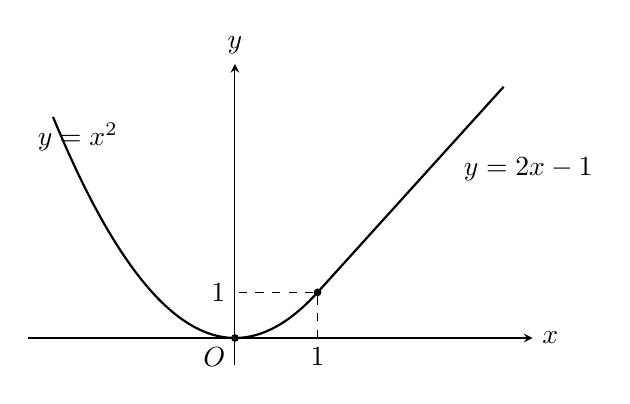
\begin{tikzpicture}[x=1.05cm,y=.58cm,>=stealth]
\draw[->](-2.5,0)--(3.6,0)node[right]{$x$};
\draw[->](0,-.6)--(0,6)node[above]{$y$};
\draw[thick,domain=-2.2:1,samples=70,smooth]plot(\x,{\x*\x});
\draw[thick](1,1)--(3.25,5.5);
\draw[dashed](1,0)--(1,1)--(0,1);
\fill(0,0)circle(1.4pt);
\fill(1,1)circle(1.4pt);
\node[below left]at(0,0){$O$};
\node[below]at(1,0){$1$};
\node[left]at(0,1){$1$};
\node at(-1.9,4.4){$y=x^2$};
\node[right]at(2.65,3.7){$y=2x-1$};
\end{tikzpicture}
\captionof{figure}{在连接点连续衔接的二次函数与一次函数}
\label{sol:fig:functions-piecewise}
\end{center}

函数值域为\([0,+\infty)\)，在\((-\infty,0]\)上严格递减，在\([0,+\infty)\)上严格递增。后一段跨过\(x=1\)仍递增，因为两侧各自递增，且连接点值相同。函数向上无界，故在\(\mathbb R\)上无界；又\(f(-1)=f(1)=1\)，因此全域没有反函数。


% ITEM: functions-power-extensions
\solutionitem{functions-power-extensions}{习题2.9（7）}
分别讨论\(x^{-2}\)、\(x^{1/3}\)、\(x^{\sqrt{2}}\)与\(x^{0}\)在基本定义域\(x > 0\)上的连续性、单调性和值域。

再讨论这些幂函数能否扩展到\(x < 0\)或\(x = 0\)，以及扩展后能否讨论奇偶性。对于无理数次幂，说明它与有理数次幂之间的联系。
\solutionanswer
在共同的定义域\((0,+\infty)\)上，四者都连续。其中\(x^{-2}\)严格递减，\(x^{1/3}\)、\(x^{\sqrt2}\)严格递增，三者的值域均为\((0,+\infty)\)；\(x^0\)恒等于\(1\)，值域为\(\{1\}\)。

扩展到其他实数时：\(x^{-2}=1/x^2\)可在\(\mathbb R\setminus\{0\}\)上定义，为偶函数，但不能在零点连续补值；\(x^{1/3}\)用实数立方根扩展到\(\mathbb R\)，在零点为\(0\)，为奇函数；\(x^{\sqrt2}\)可在零点连续补为\(0\)，通常不扩展到负半轴，故不能讨论奇偶性；\(x^0\)在非零实数上恒为\(1\)，是偶函数，作为常值函数连续延拓时可在零点补为\(1\)。

无理数次幂由正底数的有理数次幂逼近定义。上下有理逼近给出相同的极限，是这个定义不依赖所选逼近方式的保证，具体见2.3.3的题解。


% ITEM: functions-hyperbolic-functions
\solutionitem{functions-hyperbolic-functions}{习题2.9（8）}
利用双曲函数的定义完成下列问题：

\quad \exercisesubitem{1}判断\(\sinh x\)、\(\cosh x\)与\(\tanh x\)的奇偶性，并证明\(\cosh^{2} x - \sinh^{2} x = 1\)。

\quad \exercisesubitem{2}求\(\sinh x\)、\(\cosh x\)与\(\tanh x\)的值域，并判断哪些函数在\(\mathbb{R}\)上有界。

\quad \exercisesubitem{3}证明\(\sinh x\)严格递增，求其反函数；\(\cosh x\)在\(\mathbb{R}\)上是否有反函数？若限制在\([0 , + \infty)\)上，情形如何？
\solutionanswer
\exercisesubitem{1}以\(-x\)代入定义可得\(\sinh\)、\(\tanh\)为奇函数，\(\cosh\)为偶函数。又
\[
\cosh^2x-\sinh^2x
=\frac{(e^x+e^{-x})^2-(e^x-e^{-x})^2}{4}=1.
\]
\exercisesubitem{2}\(\sinh\)的值域为\(\mathbb R\)。由
\[
\cosh x-1=\frac12(e^{x/2}-e^{-x/2})^2\ge0
\]
及连续性、\(x\to+\infty\)时\(\cosh x\to+\infty\)，知其值域为\([1,+\infty)\)。令\(t=e^{2x}>0\)，则\(\tanh x=(t-1)/(t+1)=1-2/(t+1)\)，值域为\((-1,1)\)。三者中只有\(\tanh\)在全域有界。

\exercisesubitem{3}\(\sinh x=(e^x-e^{-x})/2\)的两项都随\(x\)严格递增，所以严格递增。解\(y=\sinh x\)可得反函数
\[
x=\ln\bigl(y+\sqrt{y^2+1}\bigr),\qquad y\in\mathbb R.
\]
\(\cosh\)为偶函数，故在全域不一一对应，没有反函数。限制到\([0,+\infty)\)后，令\(t=e^x\ge1\)，对\(t_2>t_1\ge1\)，有
\[
\left(t_2+\frac1{t_2}\right)-\left(t_1+\frac1{t_1}\right)
=(t_2-t_1)\left(1-\frac1{t_1t_2}\right)>0.
\]
因此此分支严格递增，反函数为\(\ln(y+\sqrt{y^2-1})\)，定义域\([1,+\infty)\)，值域\([0,+\infty)\)。


% ITEM: functions-even-odd-decomposition
\solutionitem{functions-even-odd-decomposition}{习题2.9（9）}
设\(A\)是一个关于原点对称的非空实数集合，\(f\)是\(A\)上的任意实值函数。定义
\begin{equation*}
    u(x) = \frac{f(x) + f(-x)}{2} , \qquad
    v(x) = \frac{f(x) - f(-x)}{2} .
\end{equation*}

\quad \exercisesubitem{1}证明\(u\)为偶函数，\(v\)为奇函数，且\(f = u + v\)。

\quad \exercisesubitem{2}这种“一个偶函数与一个奇函数之和”的表示是否唯一？

\quad \exercisesubitem{3}若\(f\)在\(A\)上有界，\(u\)与\(v\)是否也有界？若\(f\)连续，它们是否也连续？
\solutionanswer
\exercisesubitem{1}由于\(A\)关于原点对称，\(f(-x)\)始终有定义。直接代入得\(u(-x)=u(x)\)、\(v(-x)=-v(x)\)，并且\(u(x)+v(x)=f(x)\)。

\exercisesubitem{2}若另有\(f=U+V\)，其中\(U\)偶、\(V\)奇，则\(f(-x)=U(x)-V(x)\)。与\(f(x)=U(x)+V(x)\)相加、相减，强制得到\(U=u,V=v\)，故表示唯一。

\exercisesubitem{3}若\(|f|\le M\)，则\(|u(x)|,|v(x)|\le(|f(x)|+|f(-x)|)/2\le M\)，故两者有界。若\(f\)在\(A\)上连续，反射\(x\mapsto-x\)保持定义域，通过连续函数的复合与四则运算可知\(u,v\)也连续。


% ITEM: functions-trig-reciprocal-properties
\solutionitem{functions-trig-reciprocal-properties}{习题2.9（10）}
列出\(\tan x\)、\(\cot x\)、\(\sec x\)与\(\csc x\)的定义域、值域、奇偶性与最小正周期。

分别求这四个函数在\((0 , \pi)\)内的最大单调区间，注意将没有定义的点排除。
\solutionanswer
定义域为
\[
\begin{aligned}
D_{\tan}=D_{\sec}&=\mathbb R\setminus\{\pi/2+k\pi:k\in\mathbb Z\},\\
D_{\cot}=D_{\csc}&=\mathbb R\setminus\{k\pi:k\in\mathbb Z\}.
\end{aligned}
\]
其余性质为
\[
\begin{array}{c|c|c|c}
\text{函数}&\text{值域}&\text{奇偶性}&\text{最小正周期}\\\hline
\tan x&\mathbb R&\text{奇}&\pi\\
\cot x&\mathbb R&\text{奇}&\pi\\
\sec x&(-\infty,-1]\cup[1,+\infty)&\text{偶}&2\pi\\
\csc x&(-\infty,-1]\cup[1,+\infty)&\text{奇}&2\pi
\end{array}
\]
正割、余割平移\(\pi\)后变号，不能以\(\pi\)为周期；由其达到\(1\)的位置也可排除更小正周期。

在\((0,\pi)\)内，最大单调区间为
\[
\begin{array}{c|c|c}
\text{函数}&\text{递增区间}&\text{递减区间}\\\hline
\tan x&(0,\pi/2),\ (\pi/2,\pi)&\text{无}\\
\cot x&\text{无}&(0,\pi)\\
\sec x&(0,\pi/2),\ (\pi/2,\pi)&\text{无}\\
\csc x&[\pi/2,\pi)&(0,\pi/2]
\end{array}
\]
判断可用\(\cos x\)、\(\sin x\)的单调性与取倒数后的方向，正切、余切也可直接使用两点差公式。


% ITEM: functions-transformed-sine
\solutionitem{functions-transformed-sine}{习题2.9（11）}
设\(f(x) = 2 \sin \left( 3 x - \frac{\pi}{4} \right) + 1\)。

\quad \exercisesubitem{1}说明可以怎样从\(y = \sin x\)的图像得到\(f\)的图像，并求\(f\)的值域与最小正周期。

\quad \exercisesubitem{2}求\(f\)的最大单调增区间、最大单调减区间，以及图像的全部对称轴和对称中心。

\quad \exercisesubitem{3}判断\(f\)是否为奇函数或偶函数，并求它在\([0 , \pi]\)上取最大值的所有自变量。
\solutionanswer
\exercisesubitem{1}先把\(y=\sin x\)的横坐标压缩为原来的\(1/3\)，得到\(y=\sin3x\)；再向右平移\(\pi/12\)，纵坐标放大到\(2\)倍，最后向上平移\(1\)。值域为\([-1,3]\)，最小正周期为\(2\pi/3\)。

\exercisesubitem{2}令相位\(3x-\pi/4\)落在正弦相应的单调区间，得到全部最大单调增区间
\[
\left[-\frac\pi{12}+\frac{2k\pi}3,\frac\pi4+\frac{2k\pi}3\right],
\]
以及最大单调减区间
\[
\left[\frac\pi4+\frac{2k\pi}3,\frac{7\pi}{12}+\frac{2k\pi}3\right],\qquad k\in\mathbb Z.
\]
对称轴为\(x=\pi/4+k\pi/3\)，对称中心为\((\pi/12+k\pi/3,1)\)。

\exercisesubitem{3}\(f(0)=1-\sqrt2\ne0\)，故不是奇函数；又\(f(\pi/12)=1\ne-1=f(-\pi/12)\)，故不是偶函数。最大值\(3\)在\(x=\pi/4+2k\pi/3\)处取得，限制到\([0,\pi]\)后，全部自变量为\(\pi/4\)、\(11\pi/12\)。


% ITEM: functions-logarithmic-sine
\solutionitem{functions-logarithmic-sine}{习题2.9（12）}
设
\begin{equation*}
    f(x) = \ln \left( 3 + \sin 2 x + \sqrt{3} \cos 2 x \right) .
\end{equation*}

\quad \exercisesubitem{1}利用和差角公式化简对数内部的表达式，求\(f\)的定义域、值域与最小正周期，并说明其连续性。

\quad \exercisesubitem{2}将\(f\)限制在区间\(I = \left[ - \frac{5 \pi}{12} , \frac{\pi}{12} \right]\)上，说明为什么此时存在反函数，并求反函数及其定义域、值域。

\quad \exercisesubitem{3}求方程\(f(x) = \ln 4\)的全部实数解，并指出其中位于\(I\)内的解。
\solutionanswer
\exercisesubitem{1}有\(\sin2x+\sqrt3\cos2x=2\sin(2x+\pi/3)\)。对数内部的范围为\([1,5]\)，所以定义域为\(\mathbb R\)，值域为\([0,\ln5]\)。对数严格递增，复合后保留内层的最小正周期\(\pi\)，并在全域连续。

\exercisesubitem{2}当\(x\in I\)时，相位\(2x+\pi/3\)恰在\([-\pi/2,\pi/2]\)上。因此内层正弦及外层对数都严格递增，函数有反函数。由\(\sin(2x+\pi/3)=(e^y-3)/2\)，得
\[
f^{-1}(y)=\frac12\left[\arcsin\frac{e^y-3}{2}-\frac\pi3\right].
\]
反函数定义域为\([0,\ln5]\)，值域为\(I\)。

\exercisesubitem{3}原方程等价于\(\sin(2x+\pi/3)=1/2\)，所以
\[
x=-\frac\pi{12}+k\pi\quad\text{或}\quad x=\frac\pi4+k\pi,\qquad k\in\mathbb Z.
\]
其中位于\(I\)内的只有\(-\pi/12\)。


% ITEM: functions-trig-identities-equations
\solutionitem{functions-trig-identities-equations}{习题2.9（13）}
利用三角公式完成下列问题：

\quad \exercisesubitem{1}推导\(\sin 3 x = 3 \sin x - 4 \sin^{3} x\)。

\quad \exercisesubitem{2}证明
\begin{equation*}
    \frac{\sin \alpha + \sin \beta}{\cos \alpha + \cos \beta}
    = \tan \frac{\alpha + \beta}{2} ,
\end{equation*}
并说明等式的适用条件。

\quad \exercisesubitem{3}在\([0 , 2 \pi]\)内求解方程\(\cos 2 x = \sin x\)，以及不等式\(\sin x + \cos x \ge 1\)。
\solutionanswer
\exercisesubitem{1}由和角及二倍角公式，
\[
\begin{aligned}
\sin3x&=\sin2x\cos x+\cos2x\sin x\\
&=2\sin x\cos^2x+(1-2\sin^2x)\sin x\\
&=3\sin x-4\sin^3x.
\end{aligned}
\]
\exercisesubitem{2}令\(m=(\alpha+\beta)/2,d=(\alpha-\beta)/2\)，和差化积得
\[
\frac{\sin\alpha+\sin\beta}{\cos\alpha+\cos\beta}
=\frac{2\sin m\cos d}{2\cos m\cos d}=\tan m.
\]
条件为\(\cos\alpha+\cos\beta\ne0\)，等价于\(\cos m\cos d\ne0\)，分母及约去因子均非零。

\exercisesubitem{3}第一式化为\(1-2\sin^2x=\sin x\)，即\((2\sin x-1)(\sin x+1)=0\)。在\([0,2\pi]\)上的解为\(\pi/6,5\pi/6,3\pi/2\)。

第二式化为\(\sin(x+\pi/4)\ge1/\sqrt2\)，得到\(x\in[2k\pi,\pi/2+2k\pi]\)。与给定闭区间相交，解集为\([0,\pi/2]\cup\{2\pi\}\)。


% ITEM: functions-triangle-sas
\solutionitem{functions-triangle-sas}{习题2.9（14）}
在\(\triangle A B C\)中，\(b = 2\)，\(c = 3\)，\(A = \frac{\pi}{3}\)。

\quad \exercisesubitem{1}求边长\(a\)、三角形的面积及外接圆半径。

\quad \exercisesubitem{2}保持\(b = 2\)、\(c = 3\)不变，让\(A\)在\((0 , \pi)\)内变化。讨论边长\(a\)如何随\(A\)变化，并求面积的最大值及取到最大值时的\(A\)。
\solutionanswer
\exercisesubitem{1}由余弦定理，\(a^2=4+9-12\cos(\pi/3)=7\)，故\(a=\sqrt7\)。面积为\(S=bc\sin A/2=3\sqrt3/2\)，外接圆半径由正弦定理得到\(R=a/(2\sin A)=\sqrt{21}/3\)。

\exercisesubitem{2}当\(A\)从\(0\)增加到\(\pi\)时，\(\cos A\)严格递减，所以\(a=\sqrt{13-12\cos A}\)严格递增，取值为\((1,5)\)。面积\(S=3\sin A\)的最大值为\(3\)，恰在\(A=\pi/2\)时取得。


% ITEM: functions-triangle-ssa
\solutionitem{functions-triangle-ssa}{习题2.9（15）}
在\(\triangle A B C\)中，\(a = 1\)，\(b = \sqrt{2}\)，\(A = \frac{\pi}{6}\)。

\quad \exercisesubitem{1}这样的三角形有几个？分别求所有可能的\(B\)、\(C\)与\(c\)。

\quad \exercisesubitem{2}说明为什么由正弦定理求出\(\sin B\)之后，不能直接认定\(B\)只有一个取值，并与已知两边及其夹角的情形比较。
\solutionanswer
\exercisesubitem{1}正弦定理给出\(\sin B=(b/a)\sin A=\sqrt2/2\)。在\(0<B<\pi-A=5\pi/6\)内，两种角都可取：
\[
\begin{array}{c|c|c}
B&C&c=\sin C/\sin A\\\hline
\pi/4&7\pi/12&(\sqrt6+\sqrt2)/2\\
3\pi/4&\pi/12&(\sqrt6-\sqrt2)/2
\end{array}
\]
故共有两个三角形。

\exercisesubitem{2}在\((0,\pi)\)内，两个互补的角具有相同正弦，须继续用三角形内角和检查哪些角可取。本题两者都保留。已知两边及夹角时，余弦定理唯一确定第三边，再确定其余角，没有这里的两角选择。
\par
